\documentclass[a4paper, 12pt]{article}
\usepackage[english]{babel}
\usepackage{fullpage}
\usepackage{pgf}
\usepackage{tikz}
\usepackage{hyperref}  % makes cross references and URLs clickable
\newcommand{\code}[1]{\texttt{#1}}
\usepackage[overload]{textcase}
\usepackage{listings}
\usepackage{color}
\definecolor{light-gray}{gray}{0.95}
\usepackage{textcomp}
% set listings as in other WR-doc(s)
\lstset{columns=flexible, upquote=true, frame=single,
basicstyle=\footnotesize\ttfamily, backgroundcolor=\color{light-gray}, label=lst:init_src}
\usepackage{longtable} % table over many pages
\usepackage[document]{ragged2e} %texta djustment
\usepackage{mdwlist} % to have tight itemization
\usepackage[T1]{fontenc}
\usepackage{lmodern}
%%%%%%%%%%%%%%%%%%%%%%%%%%%%%%%%%%%%

\begin{document}
\input{version.tex}
\title{White Rabbit PTP Core User's Manual}
\author{Grzegorz Daniluk\\ CERN BE-CO-HT}

\raggedright
{\LARGE {\bf White Rabbit PTP Core User's Manual}}\\[0.2 cm]
\hrule height 4pt \vspace{0.1cm}
\raggedleft
{\large \today ~ (\gitrevinfo)}\\
{\large Building and Running}\\
\vspace*{\fill}
\raggedright
{\large Grzegorz Daniluk (CERN BE-CO-HT)}\\
\hrule height 2pt
\justify

\newpage

\tableofcontents

\newpage

{\noindent \LARGE {\bf Introduction}}\\


This is the user manual for the White Rabbit PTP Core, part of the White
Rabbit project. It describes the building and running process. If you don't
want to get your hands dirty and prefer to start with the demo binaries
available at \url{http://www.ohwr.org/projects/wr-cores/files} for officially
supported boards, please skip section \ref{Building the Core} and move forward
directly to section \ref{Programming FPGA}.


% ##########################################################################
\section{Software and hardware requirements}
\label{Software and hardware requirements}

% ==========================================================================
\subsection{Repositories and Releases}
\label{Repositories and Releases}

This manual is about the official \gitrevinfo{} stable release of the White
Rabbit PTP Core (WRPC).  The code and documentation for the project is
distributed in the following places:

\begin{itemize*}

\item \url{http://www.ohwr.org/projects/wr-cores/documents}

	hosts the pdf documentation for every official release.

\item \url{http://www.ohwr.org/projects/wr-cores/files}

	place where you can find already synthesized demo bitstreams, ready to be
  downloaded to one of the officially supported boards

\item \url{git://ohwr.org/hdl-core-lib/wr-cores.git}

	repository with the complete HDL sources of the WRPC

\item \url{git://ohwr.org/hdl-core-lib/wr-cores/wrpc-sw.git}

  repository with the LM32 software running inside the WRPC

\end{itemize*}
Other tools useful for building and running the WRPC can be downloaded from the
following locations:

\begin{itemize*}

\item \url{git://ohwr.org/misc/hdl-make.git}

  \textit{hdlmake} is used in the HDL synthesis process to create a Makefile and
  Xilinx ISE / Altera Quartus project file

\item \url{http://www.ohwr.org/attachments/download/1133/lm32.tar.xz}

  LM32 toolchain used to compile the LM32 software running inside the WRPC
  This is a 32-bit version of a toolchain. If you encounter problems running
  this toolchain on modern 64bit machines, try 64 version described below.

\item \url{http://www.ohwr.org/attachments/download/3868/lm32_host_64bit.tar.xz}

  LM32 toolchain used to compile the LM32 software running inside the WRPC
  (64-bit version of toolchain).

  \end{itemize*}
Repositories containing the WRPC gateware and software (\textit{wr-cores},
\textit{wrpc-sw}) are tagged with \texttt{wrpc-v4.0} tag. Other tools used to
build the core and load it into the FPGA should be used in their newest stable
releases, unless otherwise stated.

% ==========================================================================
\subsection{Required hardware}
\label{Required hardware}

The minimum hardware set required to run the WR PTP Core reference firmware
depends on the hardware platform you want to use. One of the following setups
can be chosen:
\begin{itemize}
  \item {\bf SPEC} PCIe board\footnote{SPEC project page
    \url{http://www.ohwr.org/projects/spec}} + FMC DIO
    card\footnote{\label{note_dio}FMC DIO project page
    \url{http://www.ohwr.org/projects/fmc-dio-5chttla}} + PC computer running
    Linux

  \item  {\bf SVEC} VME board\footnote{SVEC project page
    \url{http://www.ohwr.org/projects/svec}} + VME crate with a single board
    computer running Linux\footnote{\label{note_a20}In our test setup we used MEN A20 board}

  \item {\bf VFC-HD} VME board\footnote{VFC-HD project page
    \url{http://www.ohwr.org/projects/vfc-hd}} + FMC DIO card\footref{note_dio}
    + VME crate with s single board computer running Linux\footref{note_a20}

\end{itemize}

To be able to test White Rabbit synchronization you would also need
additional components regardless of the reference platform chosen from the list
above:
\begin{itemize}
  \item another WR node (e.g. one of the reference boards listed above or a
    White Rabbit Switch)
  \item a pair of WR-supported SFP transceivers\footnote{The list of supported
    SFPs can be found on our wiki page
    \url{http://www.ohwr.org/projects/white-rabbit/wiki/SFP}}
  \item a roll of G652, single mode fiber to connect your WR devices
\end{itemize}

% ##########################################################################
\newpage
\section{Building the Core}
\label{Building the Core}

\textbf{Note:} you can skip this chapter if you want to use the release binaries
available from \textit{ohwr.org}.

\vspace{1em}
Depending on your needs, building the WRPC can be a one- or two-step process.
In most of the cases you only need to synthesize the FPGA firmware (section
\ref{HDL synthesis}). This way, you get a working WRPC with the default, release
LM32 software running inside the core. If, for some reasons, you need to modify
the LM32 software, please check also section \ref{LM32 software compilation}
which contains a description of the software compilation process.

% ==========================================================================
\subsection{HDL synthesis}
\label{HDL synthesis}

Before running the synthesis process you have to make sure your environment is
set up correctly. You will need a synthesis software from your FPGA vendor.
Depending if you want to run the WRPC on Xilinx (e.g. SPEC, SVEC boards) or
Altera/Intel (e.g. VFC-HD) FPGA, you should install either Xilinx ISE or Quartus
Prime software.

\subsubsection{Setting up Xilinx ISE}
\label{Setting up Xilinx ISE}
To synthesize the FPGA firmware containing the WRPC, Xilinx ISE with free of
charge WebPack license is enough. ISE provides a set of scripts:
\texttt{settings32.sh}, \texttt{settings32.csh}, \texttt{settings64.sh} and
\texttt{settings64.csh} that configure all the system variables to let you
easily run the software. Depending on a shell you use and whether your Linux is
32 or 64-bits you should execute one of them before the other tools are used.
For 64-bit system and BASH shell you should call (assuming that ISE is installed
in the default \textit{/opt} directory):
\begin{lstlisting}
$ /opt/Xilinx/<version>/ISE_DS/settings64.sh
\end{lstlisting}

You can check if the shell is configured correctly by verifying if the
\texttt{\$XILINX} variable contains path to your ISE installation directory.

\subsubsection{Setting up Quartus Prime}
\label{Setting up Quartus Prime}
To be able to synthesize the WRPC for Arria V FPGA (which is used on the VFC-HD
board) you need at least a license for the Quartus Prime Standard Edition with
the support of Arria V family. To set up the software after it is installed, you
should add the location of its binaries to your \texttt{\$PATH} environment
variable. Assuming you have installed the software in \textit{/opt/altera}, the
following command should be executed:
\begin{lstlisting}
$ export PATH=/opt/altera/16.0/quartus/bin:$PATH
\end{lstlisting}

\subsubsection{Downloading the sources and running the synthesis}
Thanks to the \textit{hdlmake} tool, the synthesis process for the reference
designs does not differ between Xilinx and Intel based boards. The tool creates
synthesis Makefile as well as ISE/Quartus project file based on a set of
Manifest.py files that you will find in the \textit{wr-cores} repository.\\

First, please clone the \textit{hdlmake} repository from its location given in
section \ref{Repositories and Releases}:
\begin{lstlisting}
$ git clone git://ohwr.org/misc/hdl-make.git <your_location>/hdl-make
$ cd <your_location>/hdl-make
$ git checkout c4789c4
\end{lstlisting}
This checks out \textit{hdlmake} version 2.1 patched with the Arria V FPGA
support (VFC-HD board).

Then, using your favorite editor, you should create an \textit{hdlmake} script in
/usr/bin to be able to call it from any directory. The script should have the
following content:
\begin{lstlisting}
#!/usr/bin/env bash
python2.7 <path_to_hdlmake_sources>/hdl-make/hdlmake/__main__.py #@
\end{lstlisting}

Please, make your script executable:
\begin{lstlisting}
$ chmod a+x /usr/bin/hdlmake
\end{lstlisting}

Having all the tools in place, you can now clone the main WR PTP Core git
repository for the v4.0 release. The set of command below does that, checks out
the release tag, and downloads other HDL repositories (submodules) needed to
synthesize the core:
\begin{lstlisting}
$ git clone git://ohwr.org/hdl-core-lib/wr-cores.git <your_location>/wr-cores
$ cd <your_location>/wr-cores
$ git checkout wrpc-v4.0
$ git submodule init
$ git submodule update
\end{lstlisting}

The local copies of the submodules are stored to
\texttt{<your\_location>/wr-cores/ip\_cores}.

\vspace{1em}
\textbf{Note:} If you use the WRPC within another project (like
\textit{wr-nic}), you may need to checkout another release tag for this
repository. Please refer to the project's documentation to find out which
version of this package you need to build.

\vspace{1em}
The subdirectory you should enter to run the synthesis depends on the hardware
platform you use:
\begin{itemize*}
  \item \textbf{SPEC}: \texttt{<your\_location>/wr-cores/syn/spec\_ref\_design}
  \item \textbf{SVEC}: \texttt{<your\_location>/wr-cores/syn/svec\_ref\_design}
  \item \textbf{VFC-HD}: \texttt{<your\_location>/wr-cores/syn/vfchd\_ref\_design}
\end{itemize*}

After selecting a proper location from the list above, please call
\textit{hdlmake} without any arguments to create the Makefile and project file:
\begin{lstlisting}
$ hdlmake
\end{lstlisting}

After that, the actual synthesis is just the matter of executing:
\begin{lstlisting}
$ make
\end{lstlisting}

This takes (depending on your computer) about 10 minutes and should generate
bitstream files in various formats depending on your selected reference
hardware:
\begin{itemize*}
  \item \textbf{SPEC}: \texttt{spec\_wr\_ref\_top.bin}, \texttt{spec\_wr\_ref\_top.bit}
  \item \textbf{SVEC}: \texttt{svec\_wr\_ref\_top.bin}, \texttt{svec\_wr\_ref\_top.bit}
  \item \textbf{VFC-HD}: \texttt{vfchd\_wr\_ref.sof}
\end{itemize*}

You can select the bitstream format to be downloaded to FPGA depending on the
programming method:
\begin{itemize}
  \item \textbf{*.bin} files to program the Xilinx FPGA on SPEC or SVEC board
    using the official software support package (\textit{spec-sw},
    \textit{svec-sw}). See section \ref{Programming FPGA} for more
    information.
  \item \textbf{*.bit} files to program the Xilinx FPGA with Xilinx USB Platform
    Cable (using e.g. Xilinx Impact tool)
  \item \textbf{*.sof} file to program the Intel FPGA (VFC-HD board) using using
    the Altera / Intel JTAG cable
\end{itemize}

If, you would like to clean-up the repository to start building everything from
scratch you can use the following commands:
\begin{itemize*}
\item \texttt{\$ make clean} - removes all synthesis reports and log files;
\item \texttt{\$ make mrproper} - removes \texttt{*.bin}, \texttt{*.bit} and
  \texttt{*.sof} files;
\end{itemize*}

% ==========================================================================
\subsection{LM32 software compilation}
\label{LM32 software compilation}

\textbf{Note:} By default, the LM32 software for a stable release is embedded
inside the FPGA bitstream you've downloaded from \textit{ohwr.org} or
synthesized in section \ref{HDL synthesis}. You can skip this section, unless
you need to make some custom changes to the LM32 software and compile it
yourself.\\

First, you need to download and unpack the LM32 toolchain from the location
mentioned in section \ref{Repositories and Releases}. The following example
uses 32bit version of a toolchain. If you encounter problems running it, please
use 64bit version.
\begin{lstlisting}
$ wget http://www.ohwr.org/attachments/download/1133/lm32.tar.xz
$ tar xJf lm32.tar.xz -C <your_location>
\end{lstlisting}

Then you need to set a \texttt{CROSS\_COMPILE} environment variable in order
to compile the software for the LM32 processor:
\begin{lstlisting}
$ export CROSS_COMPILE="<your_location>/lm32/bin/lm32-elf-"
\end{lstlisting}

To get the sources of the WRPC software, please clone the \textit{wrpc-sw} git
repository tagged with \texttt{wrpc-v4.0} tag. The commands in the listing below
do that together with submodules needed for this software.\\
\begin{lstlisting}
$ git clone git://ohwr.org/hdl-core-lib/wr-cores/wrpc-sw.git \
<your_location>/wrpc-sw
$ cd <your_location>/wrpc-sw
$ git checkout wrpc-v4.0
\end{lstlisting}

\textbf{Note:} If you use WRPC within another project, you may need to checkout
a different tag or a specific commit. If this applies, please refer to a
documentation for this project.\\

Before you can compile \textit{wrpc-sw}, you can make some configuration
choices. The package uses \textit{Kconfig} as a configuration engine, so you may
run one of the following commands (the first two are text-mode, the third uses
a KDE GUI and the fourth uses a Gnome GUI):
\begin{lstlisting}
$ make menuconfig
$ make nonfig
$ make xconfig
$ make gconfig
\end{lstlisting}

Other \code{Kconfig} target applies, like \code{config}, \code{oldconfig}
and so on. A few default known-good configurations are found in
\texttt{./configs} and you choose one by \code{make}ing it by name. For all
three boards mentioned in this manual \code{spec\_defconfig} can be used.
\begin{lstlisting}
$ make spec_defconfig
\end{lstlisting}

After the package is configured, just run \code{make} without parameters to
build your binary file:
\begin{lstlisting}
$ make
\end{lstlisting}

The first time you build, the \textit{Makefile} automatically downloads
the \textit{git submodules} of this package, unless you already did that
by hand. The second and later build won't download anything
from the network.

The resulting binary \textit{wrc.bin} can be then used with the loader from
\textit{spec-sw} or \textit{svec-sw} software package to program the LM32 inside
the White Rabbit PTP Core (see section \ref{Programming FPGA} for details).

% ##########################################################################
\newpage
\section{Programming FPGA with WRPC firmware}
\label{Programming FPGA}

% ==========================================================================
\subsection{Programming FPGA on SPEC}
\label{Programming FPGA on SPEC}

\textbf{Note:} If you use a more recent version of the \texttt{spec-sw} than the
one described in this manual, the up-to-date documentation can always be found
in \textit{doc/} subdirectory of the \texttt{spec-sw} git repository.\\

First you need to clone the SPEC board software support package
(\textit{spec-sw}) from \textit{ohwr.org}. It is a set of Linux kernel drivers and
userspace tools, that interact with a SPEC board plugged into a PCI-Express
slot.\\

\begin{lstlisting}
$ git clone git://ohwr.org/fmc-projects/spec/spec-sw.git <your_location>/spec-sw
$ cd <your_location>/spec-sw
$ git checkout aff79eb
$ make
\end{lstlisting}

You have to download also the "golden" firmware for SPEC card. It is used by
the drivers to recognize the hardware:
\begin{lstlisting}
$ wget http://www.ohwr.org/attachments/download/4057/spec-init.bin-2015-09-18
$ sudo mv spec-init.bin-2015-09-18 /lib/firmware/fmc/spec-init.bin
\end{lstlisting}

Now you can load the drivers necessary to access the SPEC board from your
system:
\begin{lstlisting}
$ sudo insmod fmc-bus/kernel/fmc.ko
$ sudo insmod kernel/spec.ko
\end{lstlisting}

You can use the \textit{dmesg} Linux command to verify if this step succeeded.
Among plenty of messages you should be able to find something very similar to:
\begin{lstlisting}[basicstyle=\scriptsize\ttfamily]
[1275526.738895] spec 0000:20:00.0:  probe for device 0020:0000
[1275526.738906] spec 0000:20:00.0: PCI INT A -> GSI 16 (level, low) -> IRQ 16
[1275526.738913] spec 0000:20:00.0: setting latency timer to 64
[1275526.743102] spec 0000:20:00.0: got file "fmc/spec-init.bin", 1485236 (0x16a9b4) bytes
[1275526.934710] spec 0000:20:00.0: FPGA programming successful
[1275527.296754] spec 0000:20:00.0: mezzanine 0
[1275527.296756]       Manufacturer: CERN
[1275527.296757]       Product name: FmcDio5cha
\end{lstlisting}


By default, when loading the \textit{spec.ko} driver, FPGA gets programmed with
the "golden" bitstream. Starting from version 3.0, WR PTP Core uses a flash
memory chip on the carrier as a default place for storing the calibration
parameters and the init script. Also the storage format of this information is
now better organized in the files of the SDBFS filesystem. Therefore, starting
from v3.0 you have to write the SDBFS filesystem image to the flash
before running the WRPC. You can download the image from \textit{ohwr.org}:
\begin{lstlisting}
$ wget http://www.ohwr.org/attachments/download/4060/sdbfs-flash.bin
\end{lstlisting}

It contains all the files required by the core. They are empty, but have to
exist in the SDBFS structure to be written later as described in section
\ref{Writing configuration}. To write the filesystem image to flash, please
execute the following command:
\begin{lstlisting}
$ sudo tools/flash-write -c 0x0 0 1507712 < <your_location>/sdbfs-flash.bin
\end{lstlisting}

\noindent\textbf{Note:} If you have more than one SPEC board in your computer,
you can use \code{-b} parameter which takes the PCI bus address of the card you
want to program. This can be found in the list of the PCI devices installed in
the system (\code{lspci}).

\noindent\textbf{Note:} Please refer to section \ref{Writing SDBFS image in
standalone configuration} for instructions on how to write the SDBFS image to a
standalone SPEC or custom hardware.\\

Now, you are ready to program the FPGA with your synthesized bitstream from
\texttt{<your\_location>/wr-cores/syn/spec\_ref\_design/spec\_wr\_ref\_top.bin}
\begin{lstlisting}
$ sudo tools/spec-fwloader \
<your_location>/wr-cores/syn/spec_ref_design/spec_wr_ref_top.bin
\end{lstlisting}

If everything went right up to this moment you have your board running the FPGA 
bitstream with the WR PTP Core. If you need to load your own \texttt{wrc.bin}
compiled in section \ref{LM32 software compilation}, you can use the
\texttt{spec-cl} tool:
\begin{lstlisting}
$ sudo tools/spec-cl <your_location>/wrpc-sw/wrc.bin
\end{lstlisting}

After all these steps, you should be able to start a Virtual-UART tool (also
part of the \textit{spec-sw} package) that will be used to interact with the
WRPC shell:
\begin{lstlisting}
$ sudo tools/spec-vuart
\end{lstlisting}

If you are able to see the shell prompt \textit{wrc\#} this means the Core
is up and running on your SPEC card. Congratulations !

% ==========================================================================
\subsection{Programming FPGA on other boards}

Currently the driver packages for SVEC and VFC-HD boards depend on other CERN
drivers and front-end infrastructure. We are working to make them exportable. If
you are a CERN user of SVEC or VFC-HD board, please check
\url{https://wikis.cern.ch/display/HT/WR+Nodes} (accessible \textbf{only} from
CERN network) for more instructions. If you are outside CERN and would like to
use one of these boards, please contact us.

% ==========================================================================
\newpage
\section{Using WRPC shell}

\subsection{Writing configuration}
\label{Writing configuration}

First, you should perform a few configuration steps through the WRPC shell
before using the core.

\noindent\textbf{Note:} the examples below describe only a subset of the WRPC
Shell commands. The full list of supported commands can be found in appendix
\ref{WRPC Shell commands}.\\

Before making any configuration changes, it is recommended to stop the
PTP daemon.  Then, the messages from the daemon will not show up to the
console while you interact with the shell.

\begin{lstlisting}
wrc# ptp stop
\end{lstlisting}

\noindent First you should make sure your board has a proper MAC address
assigned:
\begin{lstlisting}
wrc# mac get
\end{lstlisting}
If the result of above command is \texttt{MAC-address: 22:33:ww:xx:yy:zz}, this
means MAC was not yet configured and stored in the Flash/EEPROM. The value is
based on thermometer serial number as is unique among SPEC devices. This is
globally accepted as ``locally assigned'', but you might want to assign your own
address. A value \texttt{22:33:44:55:66:77} is the final fallback if no
thermometer is found.

You should get the MAC for your board from its manufacturer. To configure the
address and store it into the Flash/EEPROM (so that it's automatically loaded
every time the WRPC starts) you should type two commands in the shell:
\begin{lstlisting}
wrc# mac set xx:xx:xx:xx:xx:xx
wrc# mac setp xx:xx:xx:xx:xx:xx
\end{lstlisting}
where \texttt{xx:xx:xx:xx:xx:xx} is the MAC address of your board.\\

Next, you should input calibration fixed delays values and alpha parameters. The
example below clears any existing entries and adds two Axcen transceivers with
$\Delta_{TX}$, $\Delta_{RX}$ and $\alpha$ parameters associated with them.

\begin{lstlisting}
wrc# sfp erase
wrc# sfp add AXGE-1254-0531 180625 148451 72169888
wrc# sfp add AXGE-3454-0531 180625 148451 -73685416
\end{lstlisting}

To check the content of the SFP database you can execute the \textit{sfp show}
shell command.\\

\noindent\textbf{Note:} The $\Delta_{TX}$ and $\Delta_{RX}$ parameters above are
the defaults for wrpc-v4.0 release bitstream available on \textit{ohwr.org},
running on the SPEC v4 board and calibrated to port 1 of a~WR Switch
v3.3. These values as well as the default parameters for other boards are
available on the calibration wiki page
(\url{http://www.ohwr.org/projects/white-rabbit/wiki/Calibration}). If you
re-synthesize the firmware or want to use the most accurate estimation of
the fixed delays and alpha for your fiber, you should read and perform the WR
Calibration procedure (\url{http://www.ohwr.org/documents/213}).\\

The WRPC  mode of operation (GrandMaster/Master/Slave) can be set
using the \textit{mode} command:

\begin{lstlisting}
wrc# mode gm       # for GrandMaster mode
wrc# mode master   # for Master mode
wrc# mode slave    # for Slave mode
\end{lstlisting}

This stops the PTP daemon, changes the mode of operation, but does not start it
automatically. Therefore, after calling it, you need to start the daemon
manually:

\begin{lstlisting}
wrc# ptp start
\end{lstlisting}

\noindent\textbf{Note:} For running the GrandMaster mode, you need have
\texttt{g\_with\_external\_clock\_input} generic enabled in your FPGA firmware
and provide 1-PPS and 10MHz signal from an external source (e.g. GPS receiver or
Cesium clock). Depending on your board you should connect:
\begin{itemize*}
  \item \textbf{SPEC}: DIO mezzanine LEMO No.4 for 1-PPS, LEMO No.5 for 10MHz
  \item \textbf{SVEC}: SVEC LEMO No.4 for 1-PPS, LEMO No.3 for 10MHz
  \item \textbf{VFC-HD}: DIO mezzanine LEMO No.4 for 1-PPS, LEMO No.5 for 10MHz
\end{itemize*}

\vspace{1em}
One option is to type all the commands to initialize the WRPC software to
the required state every time the core starts. However, you can also write your
own initialization script to the Flash/EEPROM. It will be executed every time
the WRPC software starts. A~simple script, that loads the calibration
parameters, configures the WR mode to Slave and starts the PTP daemon and sets
the IP address is presented below:

\begin{lstlisting}
wrc# init erase
wrc# init add ptp stop
wrc# init add sfp match
wrc# init add mode slave
wrc# init add ptp start
wrc# init add ip set 192.168.1.5
\end{lstlisting}

Almost exactly the same one can be used for running WRPC in the GrandMaster
or Master mode. The only difference would be changing the
\texttt{init add mode slave} line to \texttt{init add mode gm} or
\texttt{init add mode master}.

% ==========================================================================
\subsection{Running the Core}
\label{Running the Core}

Having the SFP calibration database, and the init script created in \ref{Writing
configuration} you can now restart the WRPC by typing the shell command:

\begin{lstlisting}
wrc# init boot
\end{lstlisting}

You should see log messages that confirm the execution of the initialization
script:

\begin{lstlisting}
executing: ptp stop
PTP stop
executing: sfp match
AXGE-3454-0531
SFP matched, dTx=180707 dRx=148323 alpha=-73685416
executing: mode slave
PTP stop
Locking PLL
executing: ptp start
PTP start
Slave Only, clock class set to 255
executing: ip set 192.168.1.5
IP-address: 192.168.1.5 (static assignment)
\end{lstlisting}

Now you should have the WR PTP Core running in WR Slave mode.\\

\textbf{Important!!!} WRPC needs to make a calibration of t24p phase transition
value. It has to be done only once for a new bitstream and is performed
automatically when WRPC runs in the Slave mode. That is why it is very
important, even if WRPC is meant to run in the Master mode, to configure it to
Slave for a moment and connect to any WR Master. This has to be repeated every
time a new bitstream (gateware) is deployed. The measured value is automatically
stored to Flash/EEPROM and used later in the Master or GrandMaster mode.\\

The Shell also contains a monitoring function which you can use to check the
WR synchronization status:

\begin{lstlisting}
wrc# gui
\end{lstlisting}

The information is presented in a clear, auto-refreshing screen. The
information is refreshed at every WR iteration or periodically if
nothing else happens (so you see an up-to-date timestamp). The period
defaults to 1 second and can be changed using the \texttt{refresh} command. To
exit from this console mode press <Esc>. A full description of the information
reporter by \textit{gui} is provied in appendix \ref{WRPC GUI elements}.

\noindent\textbf{Note:} the \textit{Synchronization status} and \textit{Timing
parameters} in \texttt{gui} are available only in the WR Slave mode. When
running as WR Master, you would be able to see only the current date and time,
link status, Tx and Rx packet counters, IP, lock and calibration status.

\vspace{1em}
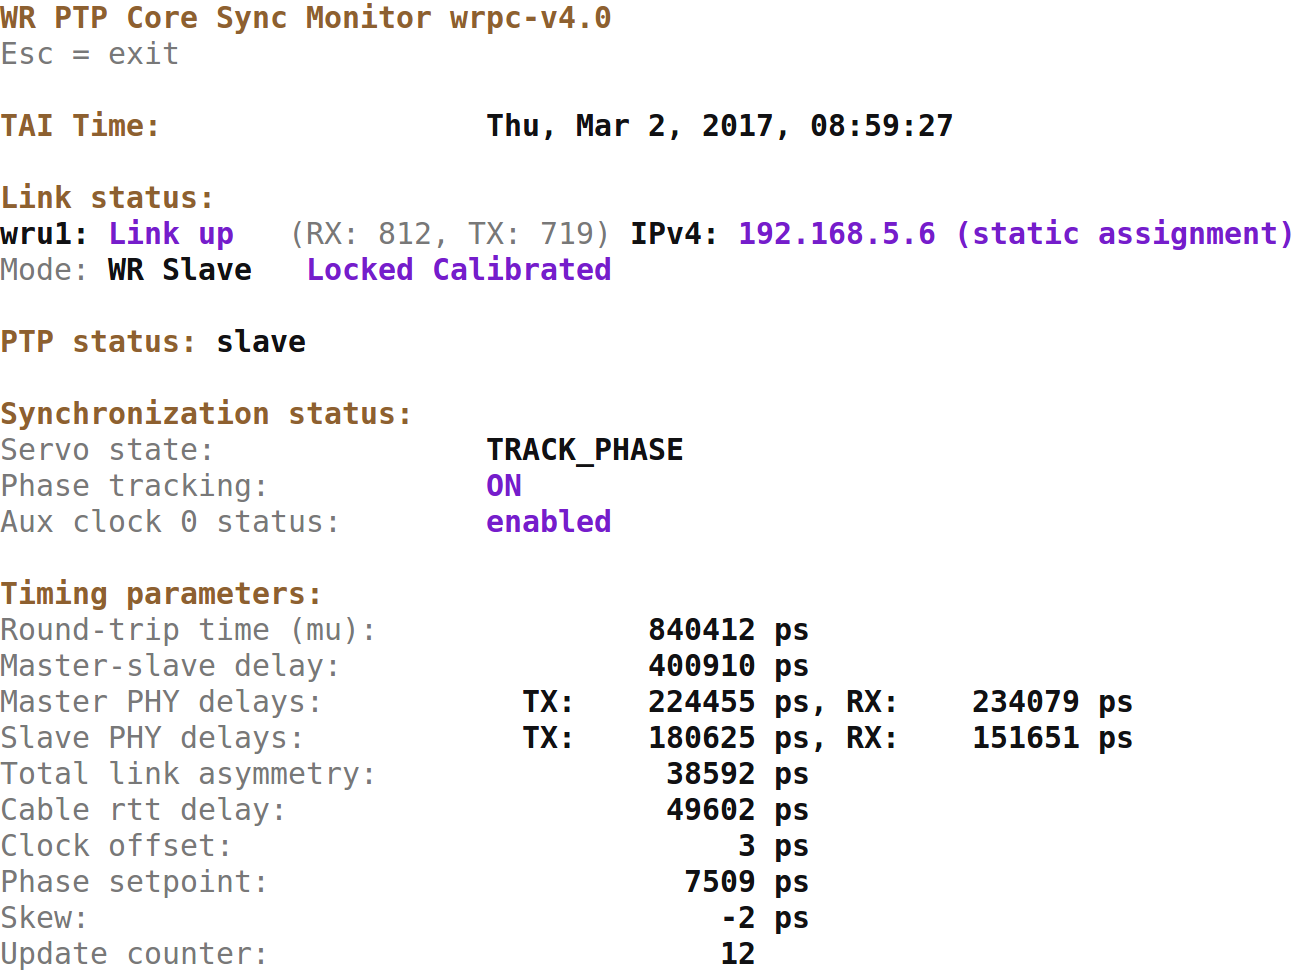
\includegraphics[width=12cm]{wrpc_mon.png}
\vspace{1em}

If you want to log statistics from the WRPC operation, it is better to use a
\texttt{stat} shell command. It reports the same information as \texttt{gui},
but in a single line, which is easier to parse and analyze:

\begin{lstlisting}
wrc# stat
lnk:1 rx:172338 tx:151811 lock:1 ptp:slave sv:1 ss:'TRACK_PHASE' aux0:1 sec:6047 \
nsec:828412744 mu:836453 dms:398530 dtxm:224455 drxm:232479 dtxs:180625 drxs:149251 \
asym:39393 crtt:49643 cko:1 setp:5082 ucnt:270 hd:31734 md:46228 ad:0 temp: 52.6875 C
lnk:1 rx:172392 tx:151860 lock:1 ptp:slave sv:1 ss:'TRACK_PHASE' aux0:1 sec:6049 \
nsec:399776360 mu:836452 dms:398530 dtxm:224455 drxm:232479 dtxs:180625 drxs:149251 \
asym:39392 crtt:49642 cko:2 setp:5082 ucnt:271 hd:31730 md:46211 ad:0 temp: 52.6875 C
(...)
\end{lstlisting}

\vspace{1em}
Unlike \texttt{gui}, the \texttt{stat} command runs asynchronously: you can still
issue shell commands while stats are running. You can stop statistics by running
\texttt{stat} again. As an alternative to the toggling action of \texttt{stat}
alone, you can use ``\texttt{stat on}'' or ``\texttt{stat off}''.

Statistics are printed every time the WR servo runs; thus no statistics
are reported when the node is running in master mode, nor when your node
is running as slave and the master disappeared.\\

You can verify the synchronization performance by observing the offset between
1-PPS signals from the WR Master and your WRPC running in the Slave mode. Please
remember to use oscilloscope cables of the same length and type (with the same
delay), or take their delay difference into account in your measurements.
Depending on your board, 1-PPS output is produced on:
\begin{itemize*}
  \item \textbf{SPEC}: DIO mezzanine LEMO No.1
  \item \textbf{SVEC}: SVEC LEMO No.1
  \item \textbf{VFC-HD}: VFC-HD LEMO L3
\end{itemize*}

% ==========================================================================
\newpage
\section{WRPC diagnostics}
\subsection{SNMP}
\label{Diagnostics via SNMP}

Up to the version 4.0 of WRPC the only way to perform diagnostics
of the \texttt{wrpc-sw} was to use serial console with tools like \textit{gui}, \textit{stat},
etc. For some set-ups, like standalone node, it is very inconvenient to use
external console for diagnostics.

From the version 4.0 of WRPC it is possible to include the \textit{Mini
SNMP responder}, which allows to perform remote diagnostics using \textit{SNMP} via
a port connected to the \textit{Write Rabbit} network.

The configuration file of WRPC contains the following
SNMP-related options:
\begin{itemize*}
\item \texttt{CONFIG\_SNMP} -- include the \textit{Mini SNMP responder} into WRPC
\item \texttt{CONFIG\_SNMP\_SET} -- enable the support of SNMP \textit{SET} packets
\item \texttt{CONFIG\_SNMP\_VERBOSE} -- enable verbose output from the \textit{Mini SNMP
      responder} on the WRPC's console
\end{itemize*}

The MIB file describing WRPC's OIDs can be found in the \texttt{lib} directory
of the \texttt{wrpc-sw} repo.
So far, the \textit{Mini SNMP responder} supports version 1 and a subset of version
2c of the SNMP protocol.
The following types of requests are supported:
\begin{itemize*}
   \item GET -- get value of a given OID
   \item GETNEXT -- get value of a next OID after the given OID (this is used
         for \texttt{snmpwalk}s)
   \item SET -- change the value of a given OID (so far used only for adding
         SFP's to the database and PTP restarts)
\end{itemize*}
The \textit{Mini SNMP responder} does not support:
\begin{itemize*}
   \item bulk requests packets (GETBULK)
   \item more than one OID in the request packet
   \item \texttt{trap} and \texttt{inform} packets
   \item encryption
   \item authentication
   \item SNMPv2c return error types; all returned error types follows SNMPv1
\end{itemize*}
To make examples more readable, listings below use \texttt{SNMP\_OPT} environment
variable. Make sure you set it properly in your shell.
\begin{lstlisting}
 $ SNMP_OPT="-c public -v 2c -m WR-WRPC-MIB -M +/var/lib/mibs/ietf:lib 192.168.1.20"
\end{lstlisting}
where:
\begin{sloppypar} % to prevent \texttt{} from going to the margine
\begin{itemize*}
   \item \texttt{-c public} -- sets SNMP community as "\textit{public}"
   \item \texttt{-v 2c} -- specifies SNMP version
   \item \texttt{-m WR-WRPC-MIB} -- specifies MIBs to be loaded
   \item \texttt{-M +/var/lib/mibs/ietf:lib} -- contains path to MIBs in the host
         system (\texttt{/var/lib/mibs/ietf}) and path to \texttt{WR-WRPC-MIB} (\texttt{lib});
         on Debian-like systems default MIBs can be downloaded using
         \texttt{download-mibs} command (package \texttt{snmp-mibs-downloader}); on
         CentOS and RedHat MIBs are included in the \texttt{libsmi} package
   \item \texttt{192.168.1.20} -- the IP address of the target board
\end{itemize*}\end{sloppypar}\noindent
For example, to get the system uptime please execute the \texttt{snmpget} command:
\begin{lstlisting}
 $ snmpget $SNMP_OPT wrpcTimeSystemUptime.0
\end{lstlisting}
To get a dump of all available OIDs please execute the \texttt{snmpwalk}
command:
\begin{lstlisting}
 $ snmpwalk $SNMP_OPT wrpcCore
\end{lstlisting}
Part of the \texttt{snmpwalk}'s output:
\begin{lstlisting}
 WR-WRPC-MIB::wrpcVersionHwType.0 = STRING: spec
 WR-WRPC-MIB::wrpcVersionSwVersion.0 = STRING: wrpc-v3.0-251-g14e952e
 WR-WRPC-MIB::wrpcVersionSwBuildBy.0 = STRING: Adam Wujek
 WR-WRPC-MIB::wrpcVersionSwBuildDate.0 = STRING: Jun  7 2016 18:12:24
 WR-WRPC-MIB::wrpcTimeTAI.0 = Counter64: 1465375022
 WR-WRPC-MIB::wrpcTimeTAIString.0 = STRING: 2016-06-08-08:37:02
 WR-WRPC-MIB::wrpcTimeSystemUptime.0 = Timeticks: (18186) 0:03:01.86
 WR-WRPC-MIB::wrpcTemperatureName.1 = STRING: pcb
 WR-WRPC-MIB::wrpcTemperatureValue.1 = STRING: 38.5625
 WR-WRPC-MIB::wrpcSpllMode.0 = INTEGER: slave(3)
 WR-WRPC-MIB::wrpcSpllIrqCnt.0 = Counter32: 1259605
 [...]
 WR-WRPC-MIB::wrpcPortSfpInDB.0 = INTEGER: inDataBase(2)
 WR-WRPC-MIB::wrpcPortInternalTx.0 = Counter32: 452
 WR-WRPC-MIB::wrpcPortInternalRx.0 = Counter32: 869
 WR-WRPC-MIB::wrpcSfpPn.1 = STRING: AXGE-1254-0531
 WR-WRPC-MIB::wrpcSfpDeltaTx.1 = INTEGER: 180625
 WR-WRPC-MIB::wrpcSfpDeltaRx.1 = INTEGER: 148451
 WR-WRPC-MIB::wrpcSfpAlpha.1 = INTEGER: 72169888
 End of MIB
\end{lstlisting}

It is recommended to use SNMP v2c for communication with a WRPC.
Please note that when the version 1 of SNMP is used, 64 bit counters are not
supported. This makes impossible to read some WRPC's objects with
SNMPv1.

% --------------------------------------------------------------------------
\subsubsection{Managing SFP database via SNMP}
\label{Managing SFP database via SNMP}

The SFPs database can be displayed using the \texttt{sfp show} command from
the WRPC's console:
\begin{lstlisting}
 wrc# sfp show
 1: PN:AXGE-1254-0531   dTx:   180625 dRx:   148451 alpha: 72169888
 2: PN:AXGE-3454-0531   dTx:   180625 dRx:   148451 alpha: -73685416
\end{lstlisting}
The same data is exported by the \textit{Mini SNMP responder} via the table
\texttt{wrpcSfpTable}:

\begin{lstlisting}
 $ snmpwalk $SNMP_OPT wrpcSfpTable
 WR-WRPC-MIB::wrpcSfpPn.1 = STRING: AXGE-1254-0531
 WR-WRPC-MIB::wrpcSfpPn.2 = STRING: AXGE-3454-0531
 WR-WRPC-MIB::wrpcSfpDeltaTx.1 = INTEGER: 180625
 WR-WRPC-MIB::wrpcSfpDeltaTx.2 = INTEGER: 180625
 WR-WRPC-MIB::wrpcSfpDeltaRx.1 = INTEGER: 148451
 WR-WRPC-MIB::wrpcSfpDeltaRx.2 = INTEGER: 148451
 WR-WRPC-MIB::wrpcSfpAlpha.1 = INTEGER: 72169888
 WR-WRPC-MIB::wrpcSfpAlpha.2 = INTEGER: -73685416
 End of MIB
\end{lstlisting}
When the SET support is compiled into the \textit{Mini SNMP responder}, it is
possible to erase or add/replace SFP entires to the SFPs database via SNMP.

\begin{sloppypar} % to prevent \texttt{} from going to the margine
Addition (or modification) of one SFP to the database can done by a row of
SNMP SETs. Firstly, please set the delta Tx (\texttt{wrpcPtpConfigDeltaTx.0}), the
delta Rx (\texttt{wrpcPtpConfigDeltaRx.0}) and the alpha (\texttt{wrpcPtpConfigAlpha.0})
with new values.
Then, to commit the change to the SFP database, perform the SNMP SET on
the \texttt{wrpcPtpConfigApply.0} with the value \texttt{writeToFlashCurrentSfp}. It will
add/update values for the currently plugged SFP.
\end{sloppypar}

To add/update entries for different SFPs, please set deltas and alpha like
above, then set PN of an SFP to the \texttt{wrpcPtpConfigSfpPn.0} and commit
the change by setting \texttt{writeToFlashGivenSfp} to the \texttt{wrpcPtpConfigApply.0}.

It is also possible to update values in the memory for the current SFP.
For that, please set delta Tx, delta Rx and alpha as described above,
then set \texttt{writeToMemoryCurrentSfp} to the \texttt{wrpcPtpConfigApply.0}

Please be aware that these changes will be lost after a power cycle of a board,
soft reset of WRPC or unplug/plug of a fiber/SFP.

Currently, after the update of SFP values in the memory, PTP is restarted.
Such restart is necessary because PTP does not support on-the-fly changes of
deltas nor alpha. It is expected that this behavior will change in the future.

If a database entry of the SFP, which is currently used was updated, it is
necessary to perform a restart of the PTP daemon
(set \texttt{wrpcPtpConfigRestart.0} with the value \texttt{restartPtp}).

Each SNMP SET of \texttt{wrpcPtpConfigApply.0} or \texttt{wrpcPtpConfigRestart.0} returns
the status of a performed action. For details please check \texttt{WR-WRPC-MIB}
file.

Commands below add an SFP with PN as "\texttt{NEW-SFP}", delta Tx "\texttt{1111}",
delta Rx "\texttt{2222}" and alpha "\texttt{3333}".
\begin{lstlisting}
 $ snmpset $SNMP_OPT wrpcPtpConfigDeltaTx.0 = 1111
 WR-WRPC-MIB::wrpcPtpConfigDeltaTx.0 = INTEGER: 1111
 $ snmpset $SNMP_OPT wrpcPtpConfigDeltaRx.0 = 2222
 WR-WRPC-MIB::wrpcPtpConfigDeltaRx.0 = INTEGER: 2222
 $ snmpset $SNMP_OPT wrpcPtpConfigAlpha.0 = 3333
 WR-WRPC-MIB::wrpcPtpConfigAlpha.0 = INTEGER: 3333
 $ snmpset $SNMP_OPT wrpcPtpConfigSfpPn.0 = NEW-SFP
 WR-WRPC-MIB::wrpcPtpConfigSfpPn.0 = STRING: "NEW-SFP"
 $ snmpset $SNMP_OPT wrpcPtpConfigApply.0 = writeToFlashGivenSfp
 WR-WRPC-MIB::wrpcPtpConfigApply.0 = INTEGER: applySuccessful(100)
\end{lstlisting}

In case the SFP database does not contain the currently plugged SFP, the last
\texttt{snmpset} command will return \texttt{applySuccessfulMatchFailed(101)}.

Optionally restart the PTP:
\begin{lstlisting}
 $ snmpset $SNMP_OPT wrpcPtpConfigRestart.0 = restartPtp
 WR-WRPC-MIB::wrpcPtpConfigRestart.0 = INTEGER: restartPtpSuccessful(100)
\end{lstlisting}

Simple verification of performed actions:
\begin{lstlisting}
 wrc# sfp show
 1: PN:AXGE-1254-0531   dTx:   180625 dRx:   148451 alpha: 72169888
 2: PN:AXGE-3454-0531   dTx:   180625 dRx:   148451 alpha: -73685416
 3: PN:NEW-SFP          dTx:     1111 dRx:     2222 alpha:     3333
\end{lstlisting}

The same add can also be achieved by performing \texttt{sfp add} command in
the WRPC's console:
\begin{lstlisting}
 wrc# sfp add NEW-SFP 1111 2222 3333
 Update existing SFP entry
 3 SFPs in DB
\end{lstlisting}

Verify the result via SNMP:
\begin{lstlisting}
 $ snmpwalk $SNMP_OPT wrpcSfpTable
 WR-WRPC-MIB::wrpcSfpPn.1 = STRING: AXGE-1254-0531
 WR-WRPC-MIB::wrpcSfpPn.2 = STRING: AXGE-3454-0531
 WR-WRPC-MIB::wrpcSfpPn.3 = STRING: NEW-SFP
 WR-WRPC-MIB::wrpcSfpDeltaTx.1 = INTEGER: 180625
 WR-WRPC-MIB::wrpcSfpDeltaTx.2 = INTEGER: 180625
 WR-WRPC-MIB::wrpcSfpDeltaTx.3 = INTEGER: 1111
 WR-WRPC-MIB::wrpcSfpDeltaRx.1 = INTEGER: 148451
 WR-WRPC-MIB::wrpcSfpDeltaRx.2 = INTEGER: 148451
 WR-WRPC-MIB::wrpcSfpDeltaRx.3 = INTEGER: 2222
 WR-WRPC-MIB::wrpcSfpAlpha.1 = INTEGER: 72169888
 WR-WRPC-MIB::wrpcSfpAlpha.2 = INTEGER: -73685416
 WR-WRPC-MIB::wrpcSfpAlpha.3 = INTEGER: 3333
 End of MIB
\end{lstlisting}

It is also possible to erase the SFPs database via SNMP (equivalent of
the \texttt{sfp erase} command):
\begin{lstlisting}
 $ snmpset $SNMP_OPT wrpcPtpConfigApply.0 = eraseFlash
 WR-WRPC-MIB::wrpcPtpConfigApply.0 = INTEGER: applySuccessful(100)
\end{lstlisting}

To verify that database is empty:
\begin{lstlisting}
 wrc# sfp show
 SFP database empty
\end{lstlisting}

% ==========================================================================
\subsection{Other Diagnostic Tools}
\label{Other Diagnostic Tools}

% --------------------------------------------------------------------------
\subsubsection{Syslog}
\label{Syslog}

\begin{sloppypar} % to prevent \texttt{} from going to the margine
The node can act as a \textit{syslog} client, though only on the UDP protocol.
To activate it, you must build with \texttt{CONFIG\_SYSLOG} and pass proper
parameters at run time.

To configure \textit{syslog} you can run the \texttt{syslog} shell command, which
receives two parameters (\texttt{ipaddr} and \texttt{macaddr}), or the
single \texttt{off} subcommand.

When deploying a network of nodes, you can choose to put the \texttt{syslog
<ip> <mac>} command in the build-time init command. To this aim you
must activate \texttt{CONFIG\_BUILD\_INIT} and then pass your command string
as \texttt{CONFIG\_INIT\_COMMAND}.  In that context, you can use ``\texttt{;}'' as
a command separator, as no newlines are permitted in \texttt{Kconfig}
strings.

The strings that a WR node sends to the \textit{syslog} server are always
using the format:  ``\texttt{<}\textit{level}\texttt{>} \textit{Jan 01 00:00:00 192.168.1.1 msg}''
where \textit{level} is usually 14 (type ``user'', priority ``info'')
and \textit{msg} is a free-format message strings.
The \textit{syslog} client sends strings to the server in the following
situations:
\begin{longtable}{  p{6.5cm}  p{9cm} }

\textit{ Boot time } &

	The node sends ``\texttt{(ma:ca:dd:rr:ee:ss) Node up since} \textit{X}
        \texttt{seconds}'' as soon as the network link is up and the \textit{syslog}
        server is configured with the shell command or init script.
        The message is re-sent, with an updated uptime value, if you change
        the \textit{syslog} server parameters. \\
& \\
\textit{ Link up after link down } &

	The message is ``\texttt{"Link up after} \textit{2.345} \texttt{s}''. The
        time printed is the duration of the link-down interval just
        passed -- no lost-by-design message is sent at link-down time. The
        message is not sent the first time the link goes up, because
        the boot message is already there.\\
& \\
\textit{ Synchronization, first time } &

	When the node reaches WR synchronization (i.e. ``track phase''
        state), it sends ``\texttt{Tracking after} \textit{5..678} \texttt{s}''.
        The reported time is the lapse since power-on.\\
& \\
\textit{ Synchronization lost } &

	Whenever WR looses \textit{track-phase} status, the node reports
        \texttt{Lost track}.\\
& \\
\textit{ Synchronization recovered } &

	When the WR servo is in \textit{track phase} state after loosing
        synchronization, the node sends ``\textit{45}\texttt{-th re-track after}
        \textit{23.456} \texttt{s}''. The time reported is the amount of time
        during which the node has not been synchronized. The seconth and
        thirth re-sync are reported as \texttt{2-th} and \texttt{3-th}, to make you
        smile. At the \texttt{4-th} you should stop smiling and be concerned.\\
& \\
\textit{ Temperature over threshold } &

	The node monitors the various thermometers every few seconds.
        If \texttt{CONFIG\_TEMP\_POLL\_INTERVAL} and related parameters are
        set, any over-temperature event is reported to \textit{syslog}.
        If any temperature in the collected set is over threshold,
        the message is ``\texttt{Temperature high:}'' followed by the list of
        all collected temperatures.  The message is repeated every
        few seconds (\texttt{CONFIG\_TEMP\_HIGH\_RAPPEL}, default 60)
        until all temperatures are under-threshold. When temperature
        is recovered the node sends ``\texttt{Temperature ok:}'' followed by
        the current list of temperatures.\\

\end{longtable}
\end{sloppypar}

% FIXME: syslog examples

% --------------------------------------------------------------------------
\subsubsection{Latency Test}
\label{Latency Test}

\begin{sloppypar} % to prevent \texttt{} from going to the margine
The configuration choice \texttt{CONFIG\_LATENCY\_PROBE} activates a
mechanism for \textit{wr} nodes to measure network latency, base on the same
hardware timestamps that are used for synchronization -- the mechanism
assumes the nodes are synchronized.

\textit{ltest} frames can be used to verify whether the network is
overloaded and/or has strange inconsistencies in node-to-node delays.

\textit{ltest} frames use a special ethernet type, \texttt{CONFIG\_LATENCY\_ETHTYPE},
which defaults to 0x0123 (291). If \textit{vlans} are active, these frames
are sent and received in the same \textit{vlans} as other CPU frames.

The \texttt{ltest} sender periodically sends three frames, with a sequence
number. One frames is at priority 7, one is at priority 6, and one is
at priority 0. The last frames reports the departure timestamps of the
previous frames.  The \textit{ltest} receiver uses ingress timestamps to
measure latency and report lost frames.

Every node built with \texttt{CONFIG\_LATENCY\_PROBE} listens for frames
belonging to \texttt{CONFIG\_LATENCY\_ETHTYPE}.  A single node in the
network is expected to send \textit{ltest} frames; use the \texttt{ltest}
shell command to select how often to send an \textit{ltest} tuple of three
frames. To enable sending every second use ``\texttt{ltest 1}'', to enable
sending every 100ms use ``\texttt{ltest 0 100}'', to stop sending use
\texttt{ltest 0}.

In the sender node, a reminder is sent to the console very 10s
reporting the node is currently sending \textit{ltest} frames.  All
non-sending nodes report every minute to \textit{syslog}. The
report message includes the number of samples received as well
as the minimum, average and maximum latency, in nanoseconds.
Any lost frames are reported both to the console and to \textit{syslog}.

You can use \textit{ltest} without \texttt{CONFIG\_SYSLOG}. In that case the
receiver nodes print the exact latency (picosecond resolution) for
every received event.
\end{sloppypar}

% --------------------------------------------------------------------------
\subsubsection{wrpc-dump}
\label{wrpc-dump}

When trying to diagnose software issues, especially lockup situations,
it may be useful to look at the current values or critical variables
within \textit{wrpc-sw}/\textit{ppsi}.

To this aim, you can pass a memory image of \textit{wrpc} to \texttt{tools/wrpc-dump}.
The tools will print information for softpll, ppsi data structures,
ptp data sets and version information.

For example, for a \textit{spec} device, you can use the resource file in
\textit{sysfs} to look at a live system, or copy the file for off-line
analysis. The following command line show both uses:

\begin{lstlisting}
   # Look for "resource0" in /sys/devices/pci, choose your bus number.
   FILE=/sys/devices/pci0000:00/0000:00:04.0/0000:04:00.0/resource0

   sudo ./tools/wrpc-dump $FILE

   sudo tools/mapper $FILE 0 0x20000 > wrpc-memory-image
   ./tools/wrpc-dump wrpc-memory-image
\end{lstlisting}

The \textit{mapper} tool used above, and part of \textit{wrpc-sw}, reads a file
using \textit{mmap()}. The kernel doesn't allow plain \textit{read()} from a
resource file. If you encounter problem using \texttt{wrpc\_dump} directly,
please use \texttt{mapper} then \texttt{wrpc\_dump}.

\textbf{Note:} Data read by \texttt{mapper} may look like has wrong endianness comparing
to the file used for programming lm32 by \texttt{spec-cl}, but \texttt{spec-cl} is the
one which change the endianness of the binary data during the programming.

With \textit{etherbone}, you can get a snapshot for \textit{wrpc} memory using
\texttt{eb-get} and the proper address (the size is always 128kB)

\begin{lstlisting}
   eb-get dev/wbm2 0x4040000/0x20000 wrpc-memory-image
   eb-get dev/ttyUSB2 0x4040000/0x20000 wrpc-memory-image
\end{lstlisting}

We won't show the 180 output lines here, to save some paper, but they
are readable dumps of the data structures, including the PTP timestamps.

% --------------------------------------------------------------------------
\subsubsection{Softpll Timing}
\label{spll Softpll Timing}

To help understanding the CPU time spent in the \textit{softpll}, you can
set \texttt{CONFIG\_SPLL\_FIFO\_LOG} in the configuration. The option
depends on \texttt{CONFIG\_DEVELOPER} and is disabled by default, because
it costs half a kilobyte in binary size and Adam is scared about any size
increase.

When the configuration option is set, \texttt{wrpc-dump} will also show
information about the last 16 \textit{softpll} iterations. Both the \texttt{tstamp}
and \texttt{duration} fields come from reading the \texttt{PPSG} nanosecond counter.

\begin{lstlisting}
   fifo log at 0x17258
        trr:                           0x0126d921
        tstamp:                        0x06b58d6a
        duration:                      0x00000c7e
        irq_count:                     2305
        tag_count:                     2304
        [... repeats for 5 more events ...]
\end{lstlisting}

% --------------------------------------------------------------------------
\subsubsection{Uptime Counter}
\label{Uptime Counter}

\textit{Wrpc-sw} now maintains an ``uptime'' counter, in seconds. It lives
at binary address 0xa0. It can be queried by \textit{etherbone}, or
seen in memory maps.

In addition to know how much as the node been up, it can be used to
know roughly when a node got stuck, and whether software is still
running when a node is not active on the network. Neither of this even
happens in production, but the tool is useful during development.

% --------------------------------------------------------------------------
\subsubsection{Profiling}
\label{Profiling}

The node now has a \textit{ps} command, that shows the number of iterations
and time spent in each \textit{task}. Each task reports when it did
something (as opposed to just polling the clock or network socket and
see nothing is there to do); the \textit{iterations} count shows how many
times the task did something.

\begin{lstlisting}
   wrc# ps
    iterations     seconds.micros    name
      44288501        4242.816329  idle
             0           0.000000  spll-bh
            37           0.016549  shell+gui
          8992           1.158969  ptp
          4252           0.037005  uptime
             1           0.001035  check-link
             0           0.000000  stats
             0           0.000000  net-bh
           568           5.068343  temperature
\end{lstlisting}

By using ``\texttt{ps reset}'' you can zero all counters to start a new
test run.

% --------------------------------------------------------------------------
\subsubsection{Pfilter rules}
\label{Pfilter rules}

By setting \texttt{CONFIG\_PFILTER\_VERBOSE}, which depends on
\texttt{CONFIG\_DEVELOPER}, you can get a dump of packet-filter rules
whenever they are activated.  This happens at initialization time and
whenever you change the MAC address or \textit{vlan} choice.

% ==========================================================================
\newpage
\section{Network Services}
\label{Network Services}

If built with \texttt{CONFIG\_IP=y}, \textit{wrpc-sw} implements the following
udp-based network services, in addition to \textit{ptp}:

\begin{longtable}{  p{6.5cm}  p{9cm} }

\textit{ bootp } &

	The node will get an IPV4 address by making \textit{bootp} queries
        once per second, until it gets a reply from a server. As an
        alternative, the address can be set using the shell command,
        and in this case the node won't send \textit{bootp} queries, or will
        stop sending them.\\
& \\
\textit{ rdate } &

	The node can be queried using \texttt{rdate -u}, once it has an IP
        address.\\
& \\
\textit{ syslog } &

	If \texttt{CONFIG\_SYSLOG} is set, the node is a syslog client.
        See section \ref{Syslog} for details.\\
& \\
\textit{ snmp } &

	If \texttt{CONFIG\_SNMP} is set, the node is a snmp agent.
        See section \ref{Diagnostics via SNMP} for details.\\

\end{longtable}

% ==========================================================================
\newpage
\section{VLAN Support}
\label{VLAN Support}

The White Rabbit node can be configured to be vlan-aware, by setting
\texttt{CONFIG\_VLAN} in \textit{Kconfig}.  The setting depends on \texttt{CONFIG\_DEVELOPER}.

If configured for \textit{vlan} support, the node select packet-filter rules
to receive frames in several \textit{vlan}s, all set at configuration time.

At run time you can use \texttt{vlan off} in the shell to turn off all \textit{vlan}
processing and get back to the ``standard'' packet-filter rules.

\begin{longtable}{  p{6.5cm}  p{9cm} }

\small{\textit{CONFIG\_VLAN}} &

	This is the top-level choice. It can be enabled or disabled.
        If disabled, the following values default to 0 and the
        packet filter will discard all tagged frames.\\
& \\
\small{\textit{CONFIG\_VLAN\_NR}} &

	The default \textit{vlan} number for the CPU.  All network traffic
        directed to (and originating from) the \textit{lm32} processor will
        belong to this \textit{vlan}.  The~value can be changed at run time
        using the \texttt{vlan} shell command.\\
& \\
\small{\textit{CONFIG\_VLAN\_1\_FOR\_CLASS7}} & \\
\small{\textit{CONFIG\_VLAN\_2\_FOR\_CLASS7}} &

	The packet-filter rules are setup to deliver frames belonging
        to two specific \textit{vlans} to class 7, usually \textit{etherbone}.
        To deliver one \textit{vlan} only, set the two options to the same
        number.\\
& \\
\small{\textit{CONFIG\_VLAN\_FOR\_CLASS6}} &

	The packet-filter rules are setup to deliver frames belonging
        to one specific \textit{vlan} to class 6, usually routed to the
        \textit{streamer} or \textit{nic} logic blocks.\\

\end{longtable}

% ##########################################################################
\newpage
\section{Troubleshooting}
\label{Troubleshooting}

\textbf{My computer hangs on loading spec.ko or programming the FPGA.}

This will occur when you try to load the driver or program the FPGA while your
\textit{spec-vuart} is running and trying to get messages from Virtual-UART's
registers inside the WRPC. Please remember to quit \textit{spec-vuart} before
reloading the driver or programming the FPGA.\\

\noindent \textbf{I want to synthesize WRPC but hdlmake says I don't have the
tools.}

If you have installed the synthesis tool (ISE for SPEC/SVEC or Quartus for
VFC-HD), but you still see the message, please make sure you have correctly set
up your environment. See sections \ref{Setting up Xilinx ISE} and \ref{Setting
up Quartus Prime} for the instructions.\\

\noindent \textbf{WR PTP Core seems to work but the 1-PPS skew on the
oscilloscope between WR Master and WR Slave is more than 1ns.}

Check if the oscilloscope cables you use have the same delays. If not, you
should either change the cables or take the delay difference into account in your
measurements. If that's not the case, please make sure you have the correct
calibration values loaded to both of your devices (see section \ref{Writing
configuration}). You made your own synthesis of the WRPC, and the default
calibration values are no longer valid, please read and perform the White Rabbit
Calibration procedure\footnote{Use the latest version of the document available
at: \url{http://www.ohwr.org/documents/213}}.

% ##########################################################################
\section{Questions, reporting bugs}
\label{Questions}

If you have found a bug, you have problems with the WR PTP Core or one of the
tools used to build and run it, you can write to our mailing list
\textbf{\textit{white-rabbit-dev@ohwr.org}}


% ##########################################################################


\appendix
\clearpage
\section{WRPC Shell Commands}
\label{WRPC Shell commands}

\footnotesize
\renewcommand\arraystretch{1.5}
\begin{longtable}{  p{7.5cm}  p{7cm} }

  \code{calibration} & (legacy) tries to read t2/4 phase transition value from
    the Flash/EEPROM (in WR Master or GrandMaster mode), or executes the t24p
    calibration procedure and stores its result to the Flash/EEPROM (in WR 
    Slave mode) \\

  \code{config} & prints the dot-config file used to build this instance of
    WRPC and ppsi. It is an optional command, enabled at build time by
    \texttt{CONFIG\_CMD\_CONFIG}. \\

  \code{delays}& \\
  \code{delays <tx> <rx>} & gets or sets the constant delays in frame
    transmission, only available if \texttt{CONFIG\_CMD\_LL}. Delays are
    expressed in picoseconds. \\

  \code{devmem <addr>} &  \\
  \code{devmem <addr> <value>} & reads or writes a 32-bit word from memory
    and/or FPGA registers. Only available if \texttt{CONFIG\_CMD\_LL} is
    set. \\

  \code{diag} & diagnostics for auxiliary user registers in HDL. Only available
    if \texttt{CONFIG\_AUX\_DIAG}.\\

  \code{diag ro <reg\_no>} & reads register <reg\_no> from read-only bank.\\

  \code{diag rw <reg\_no>} & reads register <reg\_no> from read-write bank.\\

  \code{diag w <reg\_no>} & writes register <reg\_no> from read-write bank. \\

  \code{faketemp} &  \\
  \code{faketemp <T1> <T2> <T3>} & reads or sets the three fake temperatures,
    used to test the temperature/syslog mechanism. Available if
    \texttt{CONFIG\_FAKE\_TEMPERATURES} is set. \\

  \code{gui} & starts GUI WRPC monitor \\

  \code{help} & lists available commands in this instance of the WRPC \\

  \code{init add <cmd>} & adds shell command at the end of the initialization
    script \\

  \code{init boot} & executes the script stored in Flash/EEPROM (the same
    action is done automatically when WRPC starts after resetting LM32) \\

  \code{init erase} & erases the initialization script in Flash/EEPROM  \\

  \code{init show} & prints all commands from the script stored in
    Flash/EEPROM \\

  \code{ip get} & \\
  \code{ip set <ip>} & reports or sets the IPv4 address of the WRPC (only
    available if \texttt{CONFIG\_IP} is set at build time \\

  \code{ltest} & \\
  \code{ltest fake <nsecs>} & fakes delay to trigger latency failures (for
    testing). \\

  \code{ltest <secs> <msecs>} & reads or sets the latency-test sending
    interval. See \ref{Latency Test}. Available if
    \texttt{CONFIG\_LATENCY\_PROBE} is set. \\

  \code{ltest quiet} & disables sending latency messages to Syslog. \\

  \code{ltest verbose} & enables sending latency messages to Syslog. \\

  \code{mac getp} & reads the persistent MAC address stored in Flash/EEPROM \\

  \code{mac get} & prints WRPC's MAC address \\

  \code{mac setp <mac>} & stores the persistent MAC address in Flash/EEPROM \\

  \code{mac set <mac>} & sets the MAC address of WRPC \\

  \code{mode gm|master|slave} & (legacy) sets WRPC to operate as Grandmaster
    clock (requires external 10MHz and 1-PPS reference), Master or Slave.
    After setting the mode, \texttt{ptp start} must be re-issued \\

  \code{pll cl <channel>} & checks if SoftPLL is locked for the channel \\

  \code{pll gdac <index>} & gets dac's value \\

  \code{pll gps <channel>} & gets current and target phase shift for the
    channel \\

  \code{pll init <mode> <ref\_channel> <align\_pps>} & manually runs
    \texttt{spll\_init()} function to initialize SoftPll  \\

  \code{pll sdac <index> <val>} & sets the dac \\

  \code{pll sps <channel> <picoseconds>} & sets phase shift for the channel \\

  \code{pll start <channel>} & starts SoftPLL for the channel \\

  \code{pll stop <channel>} & stops SoftPLL for the channel \\

  \code{ps} & prints the list of running tasks (processes) in the CPU. For
    each task you get the number of iterations and the CPU time consumed since
    boot or last reset of values \\

  \code{ps reset} & zeroes the profiling information reported by the \code{ps}
    command \\

  \code{ptp <e2e|p2p>} & select end-to-end PTP mechanism. If configured you can
    set \texttt{p2p} mode, and \texttt{delay}/\texttt{pdelay} as aliases. \\

  \code{ptp gm|master|slave} & sets WRPC to operate as Grandmaster clock
    (requires external 10MHz and 1-PPS reference), Master or Slave. After
    setting the mode, \texttt{ptp start} must be re-issued \\

  \code{ptp start} & starts WR PTP daemon \\

  \code{ptp stop} & stops WR PTP daemon \\

  \code{ptp <cmd> <cmd> ...} & you can concatenate several of the above
    subcommands in a single \texttt{ptp} command. With no arguments,
    the command reports the current values.\\

  \code{refresh} & changes the update time period of the gui and stat commands.
    Default period is 1 second. If you set the period to 0, the log message is
    only generated one time. \\

  \code{sdb} & prints devices connected to the Wishbone bus inside WRPC \\

  \code{sfp add <PN> <deltaTx> <deltaRx> <alpha>} & stores calibration
    parameters for SFP to a file in Flash/EEPROM \\

  \code{sfp erase} & erases the SFP database stored in the Flash/EEPROM \\

  \code{sfp match} & prints the ID of a currently used SFP transceiver and
    tries to load the calibration parameters for it \\

  \code{sfp show} & prints all SFP transceivers stored in database \\

  \code{stat} & toggles reporting of loggable statistics. You can pass
    \texttt{on} or \texttt{off} as argument as an alternative to toggling \\

  \code{stat bts} & prints bitslide value for established WR Link, needed by
    the calibration procedure \\

  \code{syslog off} &  \\
  \code{syslog <ipaddr> <macaddr>} & disables or sets your \textit{syslog}
    server. See \ref{Syslog}. Available if \texttt{CONFIG\_SYSLOG} is set. \\

  \code{temp} & reports current temperatures. \\

  \code{time} & prints current time from WRPC \\

  \code{time raw} &  prints current time in a raw format (seconds, nanoseconds) \\

  \code{time setnsec <nsec>} & sets only nanoseconds of the WRPC time \\

  \code{time setsec <sec>} & sets only seconds of the WRPC time (useful for
    setting time in GrandMaster mode, when nanoseconds counter is aligned to
    external 1-PPS and 10 MHz) \\

  \code{time set <sec> <nsec>} & sets WRPC time \\

  \code{verbose <digits>} & sets PPSi verbosity. See the PPSi manual about the
    meaning of the digits (hint: \texttt{verbose 1111} is a good first bet to
    see how the PTP system is working)  \\

  \code{ver} & prints which version of wrpc is running  \\

  \code{vlan} &  \\
  \code{vlan set <n>} & reports or sets the active vlan used for
    sending/receiving network frames. The command exists only if
    \texttt{CONFIG\_VLAN} is set.\\

  \code{vlan off} & disables vlans. Available if \texttt{CONFIG\_VLAN} is
    set. \\

  \code{w1} & lists onewire devices on the bus \\

  \code{w1w <offset> <byte> [<byte> ...]}&  \\

  \code{w1r <offset> <len>} & if \texttt{CONFIG\_W1} is set and a OneWire
    EEPROM exists, write and read data. For writing, \texttt{byte} values are
    decimal \\

\end{longtable}
\renewcommand\arraystretch{1}



% ##########################################################################
\clearpage
\section{WRPC GUI elements}
\label{WRPC GUI elements}

\footnotesize
\renewcommand\arraystretch{1.5}
\begin{longtable}{  p{4.5cm}  p{10cm} }

  \code{TAI Time:} & Current state of device's local clock \\

  \code{RX:} / \code{TX:} & Rx/Tx packets counters\\

  \code{IPv4:} & IP address; also whether it is statically configured or
    acquired via BOOTP (and the status of BOOTP) \\

  \code{mode:} & Operation mode of the WR PTP Core - \code{<WR Master,
    WR Slave>}\\

  \code{<Locked, NoLock>} & SoftPLL lock state\\

  \code{<Calibrated, Uncalibrated>} & Status of PHY calibration; not used
    anymore\\

  \code{PTP status:} & Current state of PTP state machine\\

  \code{Servo state:} & Current state of WR servo state machine -
    \code{<Uninitialized, SYNC\_SEC, SYNC\_NSEC, SYNC\_PHASE, TRACK\_PHASE>}\\

  \code{Phase tracking:} & Is phase tracking enabled when WR Slave is
    synchronized to WR Master - \code{<ON, OFF>}\\

  \code{Aux clock <N> status:} & Statuses of AUX clocks; one status line per
    available AUX clock; can contain <enabled> and <locked> \\

%   \code{Synchronization source:} & network interface name from which WR
% daemon gets synchronization - \code{<wru1>}\\

  \code{Round-trip time (mu):} & Round-trip delay in picoseconds
    ($delay_{MM}$)($delay_{MM}$)\\

  \code{Master-slave delay:} & Estimated one-way (master to slave) link
    delay ($delay_{MS}$)\\

  \code{Master PHY delays:} & Transmission/reception delays of WR 
    Master's hardware ($\Delta_{TXM}, \Delta_{RXM}$)\\

  \code{Slave PHY delays:} & Transmission/reception delays of WR Slave's
    hardware ($\Delta_{TXS}, \Delta_{RXS}$)\\

  \code{Total link asymmetry:} & WR link asymmetry calculated as
    $delay_{MM} - 2 \cdot delay_{MS}$\\

  \code{Cable rtt delay:} & Round-trip fiber latency\\

  \code{Clock offset:} & Slave to Master offset calculated by PTP daemon
  ($ offset_{MS} $)\\

  \code{Phase setpoint:} & Current Slave's clock phase shift value\\

  \code{Skew:} & The difference between current and previous estimated
    one-way link delay\\

  \code{Update counter:} & The value of a counter incremented every time
    the WR servo is updated\\

\end{longtable}
\renewcommand\arraystretch{1}


% ##########################################################################
\clearpage
\section{Writing SDBFS image in standalone configuration}
\label{Writing SDBFS image in standalone configuration}

If you use SPEC board in a host-less environment, or you use custom
hardware and SPEC drivers and tools cannot be used, there is still a
possibility of writing SDBFS through Xilinx JTAG.

\vspace{1em}
In case of SPEC running a reference bitstream provided with a stable
WRPC release, you can simply program your Flash with \textit{spec\_top.mcs}
provided with the release binaries using for example Xilinx ISE Impact tool.
This \textit{mcs} file already includes both SDBFS image and FPGA bitstream.

In case of a custom gateware or hardware, you can download a standalone
SDBFS image:
\begin{lstlisting}
$ wget http://www.ohwr.org/attachments/download/4144/sdbfs-standalone.bin
\end{lstlisting}
and generate a custom \textit{*.mcs} file with your own FPGA bitstream. You should
use the following layout:
\begin{longtable}{  l  l }
\code{0x000000} & your FPGA bitstream \\
\code{0x170000} & SDBFS image\\
\end{longtable}

For example, to generate the \textit{*.mcs} file for M25P32 Flash on SPEC, the
following \textit{promgen} parameters should be used:
\begin{lstlisting}
promgen -w -spi -p mcs -c FF -s 32768 -u 0 <your_bitstream>.bit \
-bd sdb-standalone.bin start 0x170000 -o output.mcs
\end{lstlisting}

After that, you can use the Xilinx JTAG cable and Xilinx ISE Impact tool to
write your \textit{output.mcs} file to the Flash memory.
\newpage
% ##########################################################################
\section{wrpc-dump with Older WRPC Binaries}
\label{wrpc-dump with Older WRPC Binaries}

The tool has another working mode, that you can use with older
\textit{wrpc} builds, where the special table is missing (but please be
aware that the data structures may have changed slightly).  In this
mode, you provide the address of the data structure and its name. It
supports the names \textit{pll}, \textit{fifo} (the circular log described
above), \textit{ppg}, \textit{ppi}, \textit{servo\_state}, \textit{ds} and
\textit{stats}. The \textit{ds} name
refers to the PTP data sets, and for this the pointer needed is
\texttt{ppg} (ppsi global data).
This is an example:

\begin{lstlisting}
   $ ./tools/wrpc-dump dump-file 00015798 servo_state

   servo_state at 0x15798
           if_name:                   ""
           flags:                     1
           state:                     4
           delta_tx_m:                10
           delta_rx_m:                174410
           delta_tx_s:                0
           delta_rx_s:                3200
           fiber_fix_alpha:           73622176
           clock_period_ps:           8000
           t1:                        correct 1: 1448628309.390213200:0000
           t2:                        correct 1: 1448628309.390213520:2921
           t3:                        correct 1: 1448628310.419072616:0000
           t4:                        correct 1: 1448628310.419073104:6041
   [...]
\end{lstlisting}

The address is specified as a hex number, and can be retrieved running
``\texttt{lm32-elf-nm  wrc.elf}''.

Please note that the \textit{spec} device has a strange memory mapping, and
it needs a special endian conversion. With current \textit{wrpc} it is
autodetected, but if you dump an older binary you'll need to set the
\texttt{WRPC\_SPEC} environment variable (to any value you like) to properly
access the PCI memory or a dump taken from PCI:
\begin{lstlisting}
   $ export WRPC_SPEC=y
\end{lstlisting}
or
\begin{lstlisting}
   $ WRPC_SPEC=y ./tools/wrpc-dump dump-file 00015798 servo_state
\end{lstlisting}
This is not needed if the dump is retrieved using Etherbone.

% ##########################################################################
\newpage
\section{Adding new objects to the SNMP}
\label{Adding new objects to the SNMP}

The \textit{Mini SNMP responder} can be easily expanded to export new objects.
Values of new objects can come from WRPC's variables or other HDL modules
as long as there is a proper interface to the WRPC to read these values.

This section contains the instruction how to export new objects with
the given variables' content.

The \textit{Mini SNMP responder} internally divides all OIDs into two parts.
The first part is called \textit{limb}. The \textit{limb} part of the incoming OID is
matched by a function \texttt{snmp\_respond}, with the defined \textit{limb} parts of OIDs
in the structure \texttt{oid\_limb\_array}.
When the \textit{limb} part is matched then the corresponding function from
the structure \texttt{oid\_limb\_array} is called to try to match the second part of
OID (the \textit{twig} part).

\begin{sloppypar} % to prevent \texttt{} from going to the margine
The example below adds to the \textit{Mini SNMP responder} an \texttt{int32\_t} variable
(\texttt{example\_i32var}) with OID \texttt{1.3.6.1.4.1.96.102.1.1.0} and a string
(\texttt{example\_string}) with OID \texttt{1.3.6.1.4.1.96.102.1.2.0}.
Before assigning new OIDs in your projects please contact the maintainer of
\texttt{wrpc-sw} repo to avoid conflicts.
\end{sloppypar}

\begin{itemize*}
\item First declare \texttt{example\_i32var} and \texttt{example\_string}:
\begin{lstlisting}
 static int32_t example_i32var;
 static char example_string[] = "test string";
\end{lstlisting}

\item Define the \textit{limb} part of the OID:
\begin{lstlisting}
 static uint8_t oid_wrpcExampleGroup[] = {0x2B,6,1,4,1,96,101,99};
\end{lstlisting}

\item Define the \textit{twig} part of the OID:
\begin{lstlisting}
 static uint8_t oid_wrpcExampleV1[] = {1,0};
 static uint8_t oid_wrpcExampleV2[] = {2,0};
\end{lstlisting}

\item Add a group definition to the \texttt{struct snmp\_oid\_limb oid\_limb\_array}.
      Please note that this structure has to be sorted by ascending OIDs.
\begin{lstlisting}
OID_LIMB_FIELD(oid_wrpcExampleGroup, func_group, oid_array_wrpcExampleGroup),
\end{lstlisting}
The macro \texttt{OID\_LIMB\_FIELD} takes the following arguments:
\begin{itemize*}
   \item \texttt{oid\_wrpcExampleGroup} -- an array with the \textit{limb} part of the
         OID
   \item \texttt{func\_group} -- a function to be called when the \textit{limb} part of
         the OID is matched; this function will try to match the \textit{twig} part
         of the OID within a table or a group.
   \item \texttt{oid\_array\_wrpcExampleGroup} -- an array of \textit{twig} parts of OIDs
\end{itemize*}
\item Declare a previously used \texttt{oid\_wrpcExampleGroup}. Please note that
      this structure has to be sorted by ascending \textit{twig} part of OIDs.
\begin{lstlisting}
 static struct snmp_oid oid_array_wrpcExampleGroup[] = {
   OID_FIELD_VAR(oid_wrpcExampleV1, get_p, set_p, ASN_INTEGER,   &example_i32var),
   OID_FIELD_VAR(oid_wrpcExampleV2, get_p, set_p, ASN_OCTET_STR, &example_string),
   { 0, }
 };
\end{lstlisting}
The macro \texttt{OID\_FIELD\_VAR} takes the following arguments:
\begin{itemize*}
   \item \texttt{oid\_wrpcExampleV1} -- an array with \textit{twig} part of the OID
   \item \texttt{get\_p} (or \texttt{get\_pp)} -- a function to be called when \textit{twig}
         part of the OID is matched for SNMP GET requests;
   \item \texttt{set\_p} (or \texttt{set\_pp)} -- a function to be called when a \textit{twig}
         part of the OID is matched for SNMP SET requests; if no SET
         functionality is planned, please use NULL
   \item \texttt{ASN\_INTEGER, ASN\_OCTET\_STR} -- type of the OID; please
         check the source for other possible types
   \item \texttt{\&example\_i32var, \&example\_string} -- addresses to the data in
         memory
\end{itemize*}
In case the address of variable is not known at boot, it is possible to define
a pointer to the variable which will be initialized (e.g. in the \texttt{snmp\_init}
the function) at the boot time. In that case function \texttt{get\_pp} (\texttt{set\_pp}) has
to be used instead of \texttt{get\_p} (\texttt{set\_p}). For variables that are a part of
a structure and have to be accessed via a pointer, a macro \texttt{OID\_FIELD\_STRUCT}
is available.

For more complex extraction of variables or run-time value corrections,
it is possible to use a custom \textit{get} function. It is possible to pass
a constant number to the custom function instead of an address. For example:
\begin{lstlisting}
 OID_FIELD_VAR(oid_wrpcPtpServoUpdateTime, get_servo, NO_SET, ASN_COUNTER64, \
               SERVO_UPDATE_TIME),
\end{lstlisting}

\end{itemize*}
Perform a \texttt{snmpwalk} to get new OIDs:
\begin{lstlisting}
 $ snmpwalk -On $SNMP_OPT 1.3.6.1.4.1.96.102.1
 .1.3.6.1.4.1.96.102.1.1.0 = INTEGER: 123432
 .1.3.6.1.4.1.96.102.1.2.0 = STRING: "test string"
 End of MIB
\end{lstlisting}
Trying to set too long string into the \texttt{example\_string} results in an error:
\begin{lstlisting}
 $ snmpset -On $SNMP_OPT 1.3.6.1.4.1.96.102.1.2.0 s "new long string"
 Error in packet.
 Reason: (badValue) The value given has the wrong type or length.
 Failed object: .1.3.6.1.4.1.96.102.1.2.0
\end{lstlisting}
A short enough (not longer than defined \texttt{"test string"}) value succeeds:
\begin{lstlisting}
 $ snmpset -On $SNMP_OPT 1.3.6.1.4.1.96.102.1.2.0 s "new value12"
 .1.3.6.1.4.1.96.102.1.2.0 = STRING: "new value12"
\end{lstlisting}
Set 999 to the \texttt{example\_i32var}:
\begin{lstlisting}
$ snmpset -On $SNMP_OPT 1.3.6.1.4.1.96.102.1.1.0 i 999
.1.3.6.1.4.1.96.102.1.1.0 = INTEGER: 999
\end{lstlisting}
Perform \texttt{snmpwalk} to verify changes:
\begin{lstlisting}
$ snmpwalk -On $SNMP_OPT 1.3.6.1.4.1.96.102.1
.1.3.6.1.4.1.96.102.1.1.0 = INTEGER: 999
.1.3.6.1.4.1.96.102.1.2.0 = STRING: "new value12"
End of MIB
\end{lstlisting}

% --------------------------------------------------------------------------
\subsection{Mini SNMP responder's tests}
\label{Mini SNMP responder's tests}

In the \texttt{wrpc-sw} repo, automatic tests are available to validate the \textit{Mini
SNMP responder} implementation. These tests are placed in the \texttt{test/snmp}
directory.
They use the \texttt{bats} framework (\url{https://github.com/sstephenson/bats}).

To run these tests, please go to \texttt{test/snmp} directory, then set
\texttt{TARGET\_IP} environment varaible to the IP of your target board, then type
\texttt{make}. For example:
\begin{lstlisting}
 $ TARGET_IP=192.168.1.20 make
 bats/libexec/bats snmp_tests_*.bats
   Host up 192.168.1.20
   Check the presence of snmpget
   Check the presence of snmpgetnext
   Check the presence of snmpwalk
   Check the presence of snmpset
   snmpget existing oid 1.3.6.1.4.1.96.101.1.1.1.0
 [...]
   snmpwalk 1.3.6.1.4.1.95
   snmpwalk 1.3.6 count all OIDs
 100 tests, 0 failures
\end{lstlisting}
On the left of each test there will be a tick symbol shown or an \texttt{x}
depending of the test's result (not included in the example above).

Be aware that it might be necessary to clone the \texttt{bats} repo first.
\texttt{make} command will inform whether this is needed.

In case the number of OIDs changes please correct variable \texttt{TOTAL\_NUM\_OIDS}
in file \texttt{snmp\_test\_config.bash}.

These tests have to be executed after any changes are made to the \textit{Mini SNMP
responder}.

\end{document}
